\chapter{Implementation}
\section{Application Structure}
The application consists of two main components: the frontend that presents the user with a graphical interface and the backend that provides data and actions on it to the frontend.
The user's browser connects to a web server that acts as a reverse proxy and not only provides static resources like HTML and CSS files which resemble the frontend, but also acts as a SSL endpoint.
Requests for dynamic data and actions that are handled via the REST API provided by the backend are passed on to it, its response will then be directed through the reverse proxy to the client.
To store and read data, the backend connects to a MongoDB Database. User details are synced from the existing LDAP server which acts a central repository for personal information of all employees.
TODO: Bild einfügen

\section{MongoDB}
MongoDB\footnote{https://www.mongodb.com} is a popular non-relational NoSQL Database that aims to be fast and easy to use \cite[p. 10]{MongoGuide}. To increase performance, like many NoSQL databases, it does not provide ACID\footnote{(Atomicity, Consistency, Isolation, Durability} transactions which are a well-known feature of relational database management systems (RDBMS). This, however, simplifies horizontal scaling since new machines can easily be inserted into an existing cluster of database servers without the need to be in sync. \cite[p. 3]{MongoGuide}

\subsection{BSON}
\label{BSON}
In contrast to relational databases that store all data in tables, MongoDB uses a document-orient data structure saving every element in the Binary JSON\footnote{Javascript Object Notation} (BSON) format. This approach allows complex data to be stored as one object rather than having to dissect its elements and storing them in separate tables. As a consequence, retrieving an object from the database is much more efficient than it would be using a RDBMS, as the latter needs to join the tables storing the object's nested sub-objects and compose the requested element whereas MongoDB has it stored in the exact same form it is requested. \cite[p. 10]{MongoGuide}

\subsection{Data Structure}
The application stores three diffenrent object classes in the database: Skills that are known to the system, persons with their individual contact data and skills, and sessions used to authenticate users that wish to modify their profiles. In order to instanciate the elements as java objects, Spring Data\footnote{http://projects.spring.io/spring-data/}, the framework used for database access, also stores the class name the object needs to be mapped to as a field inside of it. Furthermore, every item has the field `version' which holds a version number used to resolve writing conflicts that may occur when multiple threads access the same object simultaneously.

\subsubsection{Known Skills}
Skills known to the system consist of a uniqe name and a list of suggestions that themselves are expressed by a name and a total count of searches of the respectice suggestion together with the skill.

\begin{lstlisting}[language=JS]
{
  "_id" : "Java",
  "_class" : "com.sinnerschrader.skillwill.domain.skills.KnownSkill",
  "suggestions" : [
    {
      "name" : "AEM",
      "count" : 1
    }, {
      "name" : "jquery",
      "count" : 1
    }
  ],
  "version" : NumberLong(3)
}
\end{lstlisting}

\subsubsection{Persons}
The documents that represent persons contain the respective person's id\footnote{Each employee gets assigned an internal id (`Benutzerkürzel') that is globally used to uniquely identify a person.}, their personal data like first and last name, telephone number, e-mail address, office location, job title\footnote{The job title data is not maintained consistently in the LDAP, so that, unfortunately, it is not suitable to be used in the person search.}, and a list of the person's skills. Each of those skills consists of a name, a level of skill and a level of will.

\begin{lstlisting}[language=JS]
{
  "_id" : "foobar",
  "_class" : "com.sinnerschrader.skillwill.domain.person.Person",
  "skills" : [
    {
      "_id" : ".NET",
      "skillLevel" : 1,
      "willLevel" : 2
    },{
      "_id" : "Scrum",
      "skillLevel" : 3,
      "willLevel" : 1
    }
  ],
  "version" : NumberLong(1),
  "ldapDetails" : {
    "firstName" : "Fooberius",
    "lastName" : "Bartels",
    "mail" : "foobar@mail.org",
    "phone" : "+49 12 345678 901",
    "location" : "Hamburg",
    "title" : "Development"
  }
}
\end{lstlisting}

\subsubsection{Sessions}
Sessions are used to authenticate users that wish to modify their personal profile. The client has to authenticate the user with their credentials; if this is successful, a new session holding a unique id, the point of time it will expire, and the id of the authenticated user, will be created and stored in the database.

\begin{lstlisting}[language=JS]
{
	"_id" : "87163f310f124830bac677fe31484262",
	"_class" : "com.sinnerschrader.skillwill.session.Session",
	"username" : "foobar",
	"expireDate" : ISODate("2017-01-09T08:36:40.128Z"),
	"version" : NumberLong(1)
}
\end{lstlisting}

\subsection{Queries}
As shown in \ref{BSON}, the document based data structure of MongoDB allows the database to efficiently perform complex requests. Furthermore, it provides simple and straightforward search queries to retrieve objects based on their attributes. For example, getting all users who offer the skill `Ruby' from the collection `person' can be done with this straightforward query:
\begin{lstlisting}[language=JS]
db.person.find({ "skills._id" : "Ruby" })
\end{lstlisting}

\section{LDAP}
SinnerSchrader runs a LDAP server which acts as a centralized source of personal information of all employees. The application connects to this server in order to retrieve contact information to display in users' profiles. In comparison with having the users to enter their data manually, this methods has the benefit that the users' data will be kept in sync across all internal services, and that it reduces the effort a user has to spend to create their profile.

\section{Reverse Proxy}
Between the client and the backend, an intermediary web server that acts as a reverse proxy is switched in. Its main purpose is the distinguising between requests for static files, like HTML and CSS content that will be directly delivered by said server, and API calls that are redirected to the backend. This increases the system's security by protecting the backend server's identity and presenting an additional defense layer. \cite{NGINX}. Furthermore, this server can handle SSL encryption between the application and the client, and, if multiple backend servers are needed, balance the workload between them while presenting them as one uniform service.

\section{API}
To exchange data between the backend and the frontend, a Representational State Transfer (REST) API is provided by the backend. Its endpoints are called by the fronted code to either request data or to command the backend to perform modifying operations on it.
The used HTTP method is the main indicator of the action to perform: GET is used to retrieve data, POST to insert new elements, PUT to modify existing ones and DELETE to remove them. The URLs of the individual action express the entity on which the action will be performed.

TODO: Swagger Table in text verweisen

\begin{table}[!htp]
\centering
\rotatebox{90}{
  \begin{tabular}{l|l|l|l|l}
  URL & HTTP Method & Non-URL Parameters & Return Status & Comment\\
  \hline
  /login               & POST   & username, password                          & 200, 401, 500           & Try to login a user;\\ & & & & returns session key\\ \hline
  /logout              & POST   & session                                     & 200, 401, 500           & Logout a session\\ \hline
  /skills              & GET    & search                                      & 200, 500                & Search for autocompletion;\\ & & & & returns all skills if search is empty\\ \hline
  /skills              & POST   & name                                        & 200, 400, 401, 500      & Add new skill with\\ & & & & the given name\\ \hline
  /skills/next         & GET    & search                                      & 200, 400, 500           & Suggest a skill based on\\ & & & & the comma separated list of\\ & & & &   skills (parameter: search)\\ \hline
  /skills/\{skill\}      & DELETE &                                             & 200, 400, 401, 404, 500 & Remove the skill\\ & & & &  with the given name\\ \hline
  /skills/\{skill\}      & PUT    & name                                        & 200, 400, 401, 404, 500 & Rename the skill\\
  /users               & GET    & skills, location                            & 200, 400, 500           & Get all users\\ & & & &  matching the searched\\ & & & & skills in the given location\\ & & & & (parameters may be empty)\\ \hline
  /users/\{user\}        & GET    &                                             & 200, 404, 500           & Return the specified user\\ \hline
  /users/\{user\}/skills & POST   & session, skill, skill\_level, will\_level & 200, 400, 401, 404, 500 & Create new skill/modifiy existing\\ & & & & personal skill\\ \hline
  /users/\{user\}/skills & DELETE & session, skill                              & 200, 400, 401, 404, 501 & Remove the skill\\ & & & & from the users profile\\
  \end{tabular}
  }
\caption{Lasers in space!}
\end{table}



\section{Backend}
The backend component ist implemented in Java 8\footnote{https://go.java/} using the Spring Boot framework\footnote{https://projects.spring.io/spring-boot/}. Maven\footnote{https://maven.apache.org/what-is-maven.html} is employed to manage the build process and run unit and integration tests.

\section{Architecture}
The software architecture consists of three main categories of classes: services handling data manipulation and filtering that hold the business logic, repository objects that wrap the database operations into easy-to-use handlers, and domain specific data types. Additionally, numerous helper classes like custom exception types, comparators and general utilities are implemented.

// TODO UML und paste

\subsection{Spring Boot}
Spring Boot is a highly sophisticated web framework that provides numerous features to create web applications including, but not limted to, annotations to expose java methods as HTTP request endpoints, an embedded webserver to run the application on, a modular design to extend its features, and annotation based dependency injection. It is used because its credo to provide default configurations where possible and thus reduce the need to write infrastructure code simplifies the applications structure.\cite[p. 6]{SpringGuide}
For example, a controller that returns a static response can be created using two annotations:
`@Controller' to make spring boot identify the class as a resource that will listen to HTTP calls, and `@Request' to specify the URL and HTTP method to use. Unlike most other web frameworks, spring boot does not require any more configuration or dispatching classes.

\begin{lstlisting}[language=Java]
@Controller
public class HTCPCPImpl {

	@RequestMapping(path = "/coffee", method = RequestMethod.GET)
	public ResponseEntity<String> coffee() {
		StatusJSON json = new StatusJSON("I'm a teapot \u2615");
		return new ResponseEntity<String>(
      json.toString(),
      HttpStatus.I_AM_A_TEAPOT
    );
	}

}
\end{lstlisting}

\subsection{Spring Data Repositories}
Spring Data\footnote{http://projects.spring.io/spring-data/} is a module for Spring Boot that streamlines the way elements can be accessed from a database.
The component mainly used in this application are CRUD\footnote{Create, Read, Update, Delete} repository objects that enclose the database connections and serve
simple java methods as an interface. To create such a repository, a java interface defining the stored data type and custom database queries has to be constructed.
No actual implementation of the interface has to be created since it will be generated automatically by Spring Data.
The parameters needed to connect to the database have to be configured in any source of properties known to Spring Boot, e.g. in `src/main/resources/application.properties'.

\begin{lstlisting}[language=Java]
public interface PersonRepository
    extends MongoRepository<Person, String> {

	Person findById(String id);

	@Query("{ skills._id : ?0 }")
	List<Person> findBySkill(String skillName);

}
\end{lstlisting}

\begin{lstlisting}[language=Java]
spring.data.mongodb.host=127.0.0.1
spring.data.mongodb.port=27017
spring.datasource.driverClassName=com.mongodb.Mongo
\end{lstlisting}

\subsection{Swagger}
Swagger\footnote{http://swagger.io/} is an open-source framework for creating documentations of REST APIs.
Its annotation based java integration is heavily used to generate an interactive overview of the API endpoints provided by the
backend. This overview is automatically served by spring boot and contains a list of all URLs to make requests to, HTTP response codes to expect, the content type of the response and an built-in form to make example requests. The main advantage of this approach is that the code and its documentation are located at the very same place and that parts of the documentation are automatically gernerated, so that the both are maintained synchronously, thus avoiding the documentation differing from the implementation.
\begin{figure}[!htp]
    \centering
    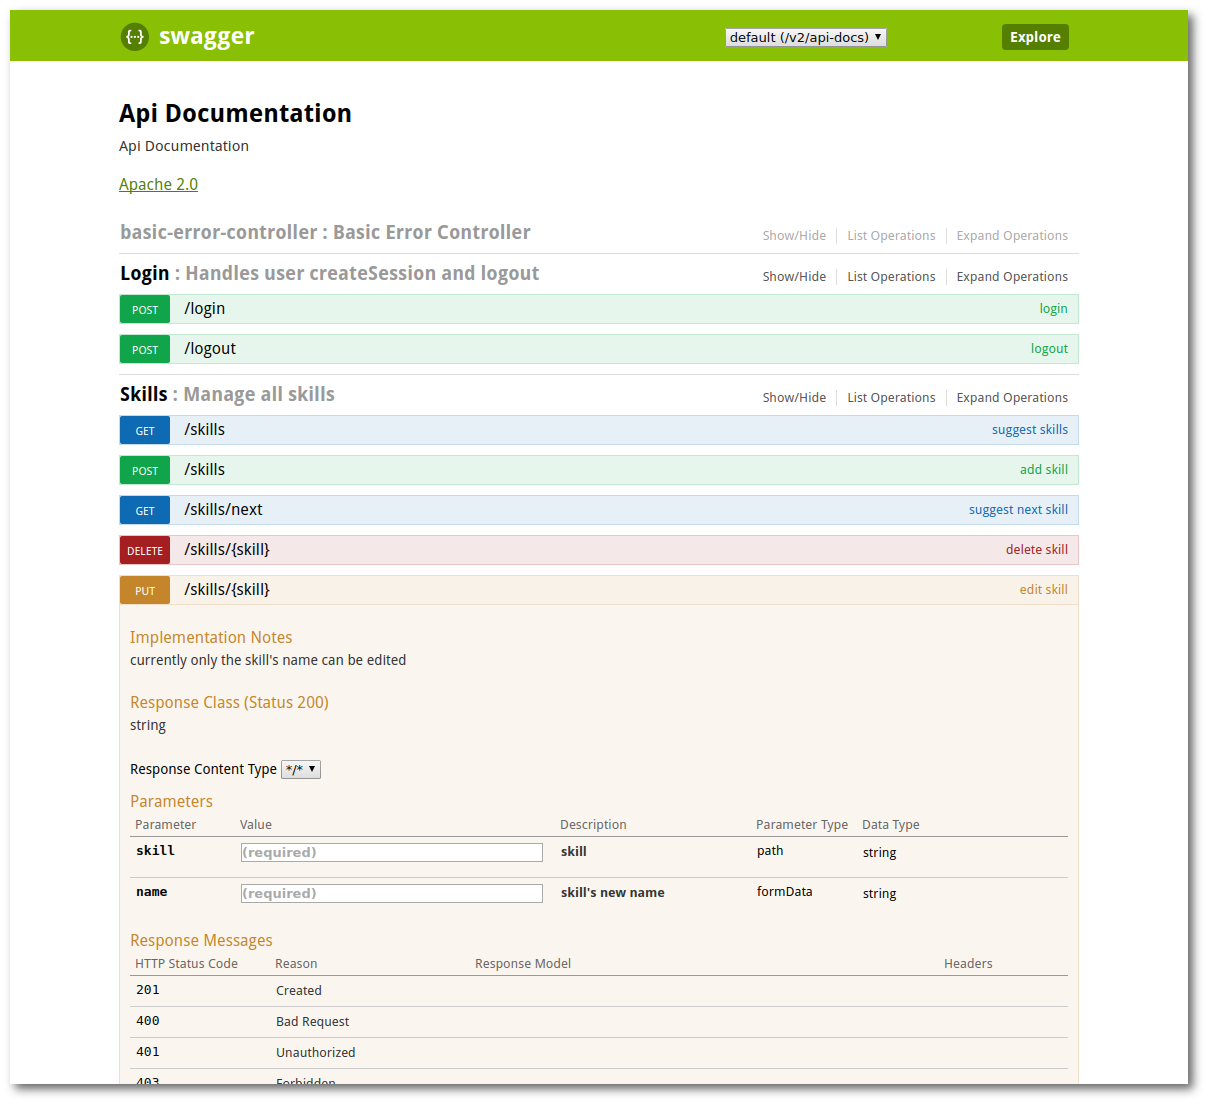
\includegraphics[width=\textwidth]{images/swagger_ui.png}
    \caption[Swagger Interactive Documentation]{Interactive API documentation generated by Swagger}
    \label{fig:markovchain}
\end{figure}

\subsection{Testing}
As a part of the build process, automatic tests are run using the JUnit\footnote{http://junit.org} framework. Two types of tests are employed to ensure the proper working of the software: unit tests that validate isolated segments (java classes), and integration tests that simulate calls to the controllers and test the
interplay of the individual components.

\subsubsection{Embedded Services}
During the integration test phase, external services like LDAP and a database have to be accessed in order to ensure the proper working of the interfaces connecting to them. Using the real services, however, is not an option as it cannot be assumed that the machine that runs the tests has a connection to them, and because the tests have to take control over the state of the services. To solve this, a LDAP server and a MongoDB are embedded into the application and will be used during testing.
The embedded database is the MongoDB implementation by `flapdoodle'\footnote{https://github.com/flapdoodle-oss/de.flapdoodle.embed.mongo}, which has the advantage of being effortlessly deployed by importing it; all further configuration and setup happen automatically. As an embedded LDAP, the implementation created for the `unboundid' framework\footnote{https://www.ldap.com/unboundid-ldap-sdk-for-java} is used.

\section{License}
The software is licensed under the MIT license \cite{license} which is considered one of the most popular open source licenses, mainly because it grants a high level of freedom to modify and use the software under the sole condition that a copy of the original license is distributed algonside the software.

\begin{quote}
Copyright 2017 SinnerSchrader Deutschland GmbH

Permission is hereby granted, free of charge, to any person obtaining a copy of this software and associated documentation files (the "Software"), to deal in the Software without restriction, including without limitation the rights to use, copy, modify, merge, publish, distribute, sublicense, and/or sell copies of the Software, and to permit persons to whom the Software is furnished to do so, subject to the following conditions:

The above copyright notice and this permission notice shall be included in all copies or substantial portions of the Software.

THE SOFTWARE IS PROVIDED "AS IS", WITHOUT WARRANTY OF ANY KIND, EXPRESS OR IMPLIED, INCLUDING BUT NOT LIMITED TO THE WARRANTIES OF MERCHANTABILITY, FITNESS FOR A PARTICULAR PURPOSE AND NONINFRINGEMENT. IN NO EVENT SHALL THE AUTHORS OR COPYRIGHT HOLDERS BE LIABLE FOR ANY CLAIM, DAMAGES OR OTHER LIABILITY, WHETHER IN AN ACTION OF CONTRACT, TORT OR OTHERWISE, ARISING FROM, OUT OF OR IN CONNECTION WITH THE SOFTWARE OR THE USE OR OTHER DEALINGS IN THE SOFTWARE.
\end{quote}\cite{license}
